


\documentclass[10pt,a4paper]{article}

% ------------------------------------------------
% ZAKLADNI NASTAVENI A BALICKY
% ------------------------------------------------
\usepackage[T1]{fontenc}
\usepackage[utf8]{inputenc}
\usepackage[czech]{babel}
\usepackage{lmodern}
\usepackage[a4paper,margin=2.3cm,headheight=14pt]{geometry}

\usepackage{pdflscape}
\usepackage{microtype}
\usepackage{graphicx}
\usepackage{float}
\usepackage{booktabs}
\usepackage{tabularx}
\usepackage{longtable}
\usepackage{array}
\usepackage{enumitem}
\usepackage{fancyhdr}
\usepackage{xcolor}
\usepackage{listings}
\usepackage{tikz}
\usetikzlibrary{arrows.meta,positioning,shapes.geometric,automata}

\usepackage[hidelinks]{hyperref}

% ------------------------------------------------
% VZHLED DOKUMENTU
% ------------------------------------------------
\setlength{\parindent}{0pt}
\setlength{\parskip}{4pt}
\setlist{nosep,leftmargin=*}

\pagestyle{fancy}
\fancyhf{}
\lhead{IFJ26 -- Dokumentace projektu}
\rhead{\thepage}
\renewcommand{\headrulewidth}{0.4pt}

\hypersetup{
    pdftitle={Dokumentace projektu IFJ26},
    pdfsubject={Implementace překladače imperativního jazyka IFJ26}
}

% Sloupec s automatickým zalamováním textu
\newcolumntype{Y}{>{\raggedright\arraybackslash}X}

% ------------------------------------------------
% UDAJE K DOPLNENI
% ------------------------------------------------
\newcommand{\nazevprojektu}{Implementace překladače imperativního jazyka IFJ26}
\newcommand{\varianta}{vv-BVS}
\newcommand{\gitrepo}{https://github.com/martin-yeaaa/prekladac-ifj26}

\begin{document}

% =================================================
% TITULNI STRANA
% =================================================
\begin{titlepage}
    \centering
    {\large VYSOKÉ UČENÍ TECHNICKÉ V BRNĚ}\\[0.3cm]
    {\large Fakulta informačních technologií}\\[2.0cm]

    {\Large Dokumentace projektu}\\[0.5cm]
    {\huge\bfseries \nazevprojektu}\\[1.5cm]

    \begin{tabularx}{\textwidth}{|l|Y|Y|Y|}
        \hline
        \textbf{Člen týmu} & \textbf{VUT login} & \textbf{Osobní číslo} & \textbf{Podíl bodů} \\
        \hline
        \textbf{Martin Vaško} & xvaskom00 & 282244 & 54 \% \\
        \hline
        Michal Bína & xbinami00 & 282028 & 13 \% \\
        \hline
        Lukáš Dvořák & xdvoral00 & 282092 & 20 \% \\
        \hline
        Jiří Švec & xsvecji00 & 281993 & 13 \% \\
        \hline
    \end{tabularx}

    \vspace{1.0cm}
    \begin{tabularx}{\textwidth}{lY}
        \textbf{Varianta zadání:} & \varianta \\
        \textbf{Implementovaná rozšíření:} &ŽÁDNÁ \\
        \textbf{Git repozitář:} & \url{\gitrepo} \\
    \end{tabularx}

    \vfill
    {\large Brno, 2026}
\end{titlepage}

\tableofcontents
\newpage

% =================================================
\section{Rozdělení práce}
% =================================================
% Uvedte, kdo se podilel na jednotlivych castech projektu.
% Pokud rozdeleni bodu neni rovnomerne, uvedte jeho duvod.

\subsection{Členové týmu a jejich odpovědnosti}

\begin{itemize}
    \item \textbf{xvaskom00:} implementace celého parseru a sémantické analýzy, tabulky symbolů a BVS, specifikace AST, nárvh a oprava gramatiky
    \item \textbf{xdvoral00:} generátor kódu 
    \item \textbf{xbinami00:} část lexeru a část gramatiky a tabulky
    \item \textbf{xsvecji00:} část lexeru a dokumentace
\end{itemize}

\subsection{Odůvodnění rozdělení bodů}
Rozdělení bodů bylo přizpůsobeno podle vykonané práce každého člena a také podle jejich přístupu k práci.

% =================================================
\section{Spolupráce a vývoj}
% =================================================
\subsection{Organizace spolupráce a verzování}
Jako komunikační prostředek byl zvolen \texttt{Discord}. Neukázal se však jako dostačující, protože někteří členové týmu na zprávy reagovali později, než bylo potřeba.

Důležité věci se probraly na 2 offline schůzkách a 2 online schůzkách.

Pro verzování byl využit \texttt{github}. 



\subsection{Code review a schvalování změn}
Code review byl prováděn samostatně s pomocí AI nástrojů.

\subsection{Testování}
Některé části byly testovány ručně, jiné pomocí testovací knihovny \texttt{GoogleTest}.

\subsection{Formátování zdrojového kódu}
K formátování zdrojového kódu byl využit \texttt{clang-format LLVM}. \\
Pro názvy identifikátorů byl použit \texttt{snake\_case}, pro klíčová slova (typedef) \texttt{PascalCase} . Pro výčty (enum) a konstanty byl použit \texttt{MACRO\_CASE}.

% =================================================
\section{Architektura řešení}
% =================================================
% Vlozte vlastni blokove schema. Diagram musi ukazovat moduly,
% datove toky a struktury predavane mezi moduly.

\subsection{Blokové schéma}

% Moznost vlozeni externiho obrazku:
% \begin{figure}[H]
%     \centering
%     \includegraphics[width=\textwidth]{architektura.pdf}
%     \caption{Blokové schéma architektury překladače}
%     \label{fig:architektura}
% \end{figure}

% Nebo vytvorte diagram primo v TikZ:
\begin{figure}[H]
    \centering
    \fbox{\parbox[c][5cm][c]{0.9\textwidth}{
        \centering
        ZDE VLOŽTE BLOKOVÉ SCHÉMA ARCHITEKTURY
    }}
    \caption{Blokové schéma architektury překladače}
    \label{fig:architektura}
\end{figure}

\subsection{Popis datových toků a komponent}
DOPLŇTE VLASTNÍ TEXT.

% =================================================
\section{Lexikální analýza}
% =================================================
\subsection{Konečný automat}

\begin{landscape}
\begin{figure}[p]
    \centering
    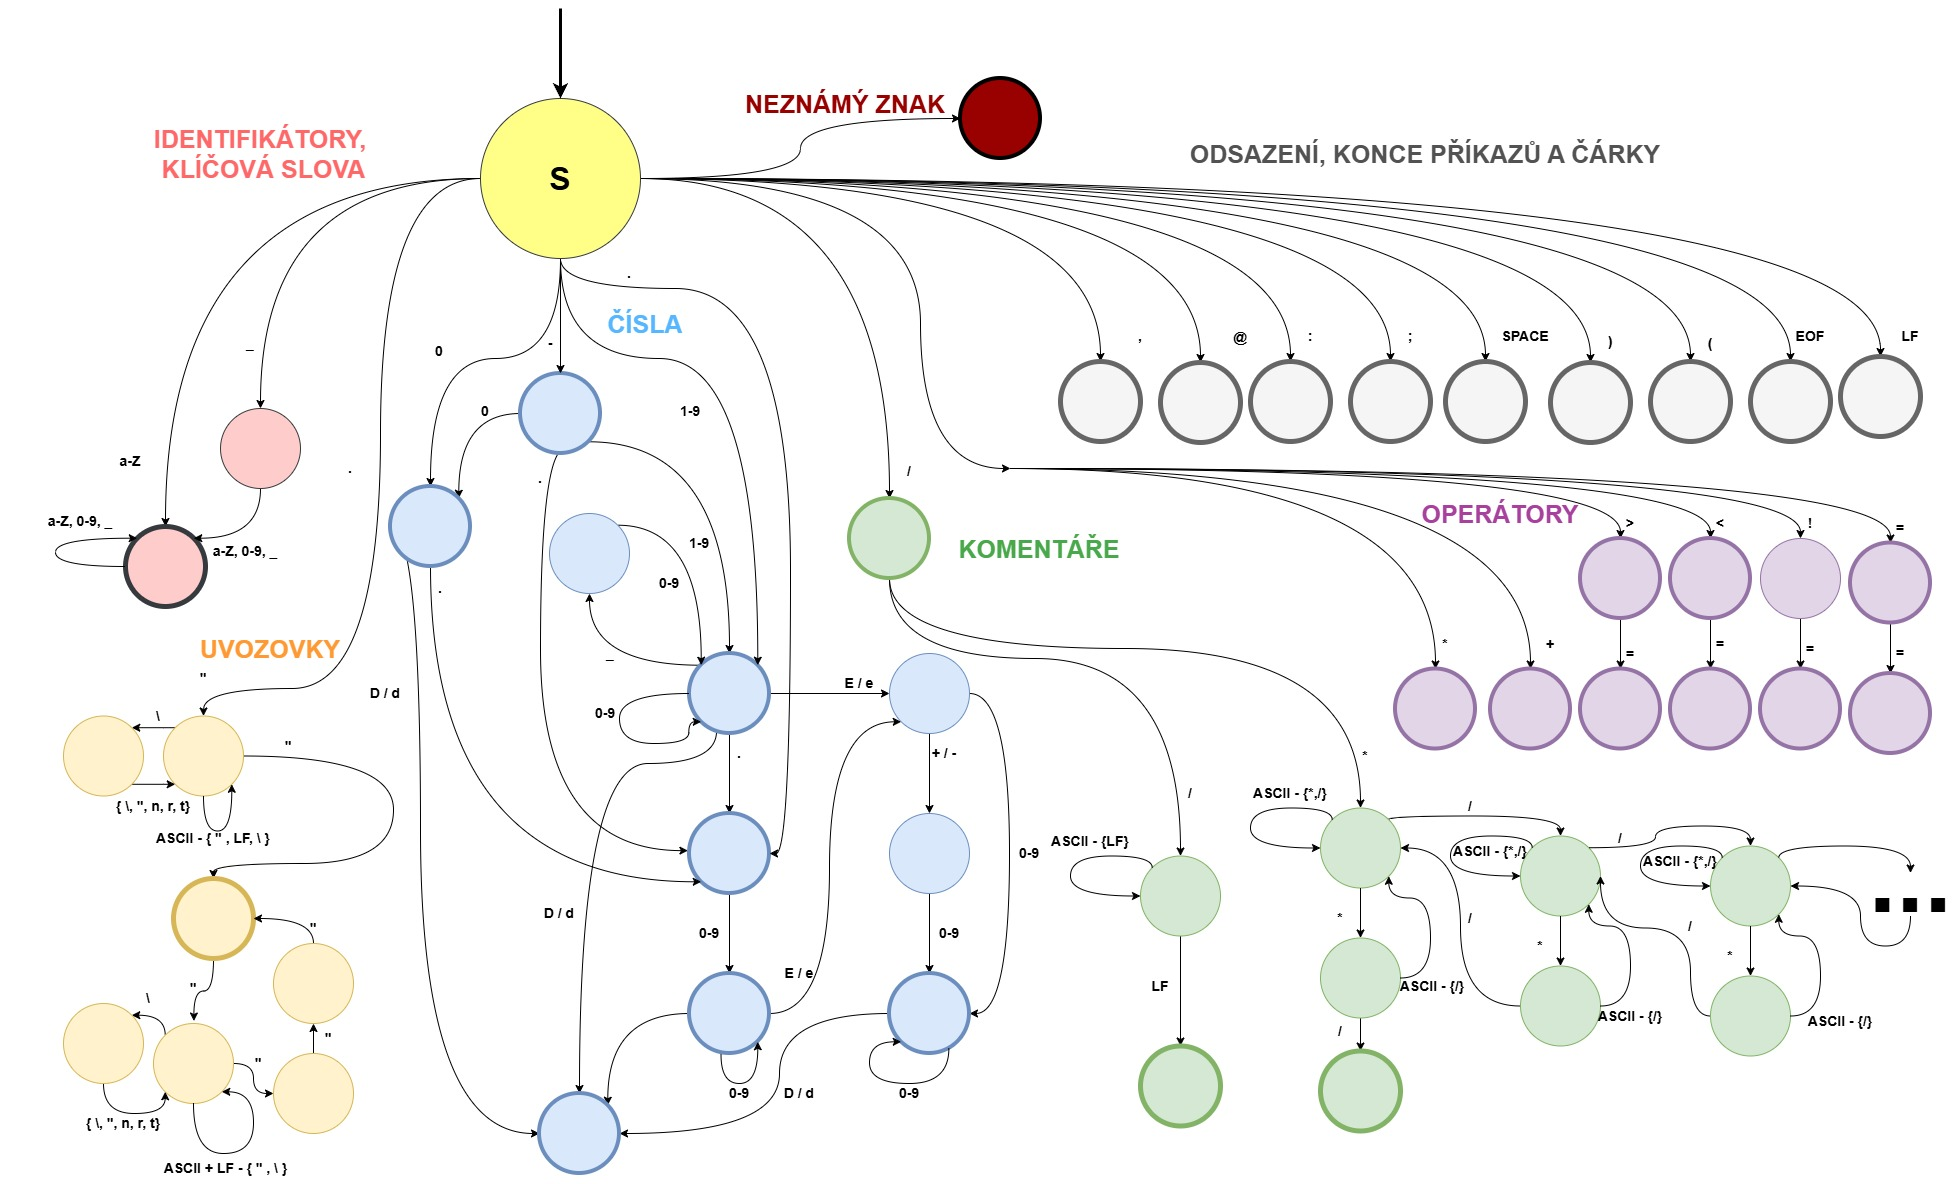
\includegraphics[
        width=0.95\linewidth,
        height=0.85\textheight,
        keepaspectratio
    ]{FSM_ver5.jpg}
    \caption{Konečný automat lexikálního analyzátoru}
    \label{fig:automat}
\end{figure}
\end{landscape}

\subsection{Odchylky od standardního modelu}
1. Token pro \texttt{@} byl nakonec řešen jinak (jako celek \texttt{@main)}. \\
2. Mezery, \texttt{LF} a \texttt{EOF} mají vlastní pravidla. \\
3. Diagram dovoluje pouze jedno podtržítko mezi číslicemi, ale implementace dovoluje více. \\
4. Vnořené komentáře jsou řešeny složitěji a v diagramu by šly těžko zapsat.

% =================================================
\section{Syntaktická analýza}
% =================================================
\subsection{LL gramatika}
% ZDE VLOZTE VLASTNI GRAMATIKU.

\subsection{LL tabulka}
% Tabulku vytvorte podle vlastni gramatiky.
% Pro rozsahlejsi tabulku lze pouzit longtable.

\begin{table}[H]
    \centering
    \caption{LL tabulka}
    \label{tab:ll}
    \begin{tabular}{c|c}
        \toprule
        \textbf{Neterminál} & \textbf{DOPLŇTE TERMINÁLY A PRAVIDLA} \\
        \midrule
        DOPLŇTE & DOPLŇTE \\
        \bottomrule
    \end{tabular}
\end{table}

\subsection{Precedenční tabulka}
% ZDE VLOZTE VLASTNI PRECEDENCNI TABULKU.
% U rozsahle tabulky upravte sirku a velikost pisma podle potreby.

\begin{table}[H]
    \centering
    \caption{Precedenční tabulka}
    \label{tab:precedence}
    \begin{tabular}{c|c}
        \toprule
        \textbf{Terminál} & \textbf{DOPLŇTE ZNAKY PRECEDENCE} \\
        \midrule
        DOPLŇTE & DOPLŇTE \\
        \bottomrule
    \end{tabular}
\end{table}

% =================================================
\section{Popis implementovaných modulů}
% =================================================
% Pro kazdou dvojici .c/.h uvedte kratky, vecny popis.
% Radky podle potreby pridejte nebo odeberte.

\begin{longtable}{p{0.30\textwidth}p{0.68\textwidth}}
    \toprule
    \textbf{Modul} & \textbf{Stručný popis odpovědnosti modulu} \\
    \midrule
     \texttt{lexer.c / lexer.h} & Ze zdrojového kódu v jazyce \texttt{IFJ26}, který si celý zanalyzuje, umožnuje postupně vrátit všechny vytvořené tokeny z programu.  \\
     \texttt{parser.c / parser.h / } & Nad tokeny, které si vezme od lexeru, provede syntaktickou analýzu a vytvoří odpovídající abstraktní syntaktický strom. \\
     \texttt{semantics.c / semantics.h} & Z BST kontroluje, zda je program sémanticky správně a vrací abstraktní sémantický strom.\\
     \texttt{symtable.c / symtable.h} & DOPLŇTE \\
     \texttt{codegen.c / codegen.h} & Modul codegen prochází výsledný AST strom a generuje z něj cílový mezikód .IFJcode26, přičemž pro výpočty výrazů používá datový zásobník a pro každou funkci vytváří vlastní lokální rámec (LF)\\
     \texttt{bst.c / bst.h / bst\_priv.h} & Umožnuje ukládat data do výškově vyváženého binárního stromu a poté k nim efektivně přistupovat. \\
    \texttt{error\_codes.h} & Obsahuje seznam chybových návratových kódů. \\
     
    \bottomrule
\end{longtable}


% =================================================
\section{Využití nástrojů AI}
% =================================================
% Podle zadani uvedte konkretni nastroje a modely, typicky postup,
% problemy a priklady navrhu, ktere jste nevyuzili nebo upravili.
% Tuto cast vyplnte vlastnimi skutecnymi zkusenostmi.

\subsection{Použité nástroje a modely}
- ChatGPT
\\
- Claude Sonet 5.5 Medium Effort
\\
- Gemini

\subsection{Pracovní postup}
Dovysvětlení zadání a funkci dílčích částí překladače, k vyplnění jednoduchých polí podle předlohy a ke konzultaci našeho řešení. \\
Dále byl využit k tvorbě šablony pro tuto dokumentaci.
\\
\\
Dovysvětlení k čemu slouží abstraktní syntaktický strom a k čemu slouží tabulka symbolů, tvorba testovací sady pro modul \texttt{semantics}, po dokončení daného modulu hledání chyb v kódu parseru, semantické analýzy, a tabulky symbolů.\\

\subsection{Problémy a nevyužité nebo upravené návrhy}
- Na vysvětlení věcí bylo potřeba se ptát vícekrát, protože AI vysvětlovalo příliš složitě.\\
- Při hledání chyb AI vypisovalo i chyby které ve skutečnosti chybami nebyly.
\\
- Testy pro modul \texttt{semantics} bylo potřeba psát vícekrát, protože AI správně nevytvořilo \texttt{AST} podle naší konkrétní specifikace. 
\\
- Byla využívána bezplatná verze, takže občas došly tokeny a bylo potřeba čekat.
\\

\end{document}




